\chapter{\bevezetes}

A digitalizáció hatására ma, már minden háztartásban található vezetékes és vezeték nélküli eszköz is hozzáfér az internethez, melynek nemcsak előnye, de hátránya, hogy ezek ugyanolyan veszélynek vannak kitéve, mint bármely más, kisebb vagy nagyobb cégekhez tartozó üzleti hálózatok. Szeretném bemutatni a hálózatok működésének alapfogalmait és az okos otthoni hálózatban résztvevő eszköztípusokat, feltárom azokat a sérülékenységi lehetőségeket, melyek nagy szerepet játszanak abban, hogy eljussunk a teljesen biztonságos lakhatáshoz.
\begin{figure}[!ht]
    \centering
    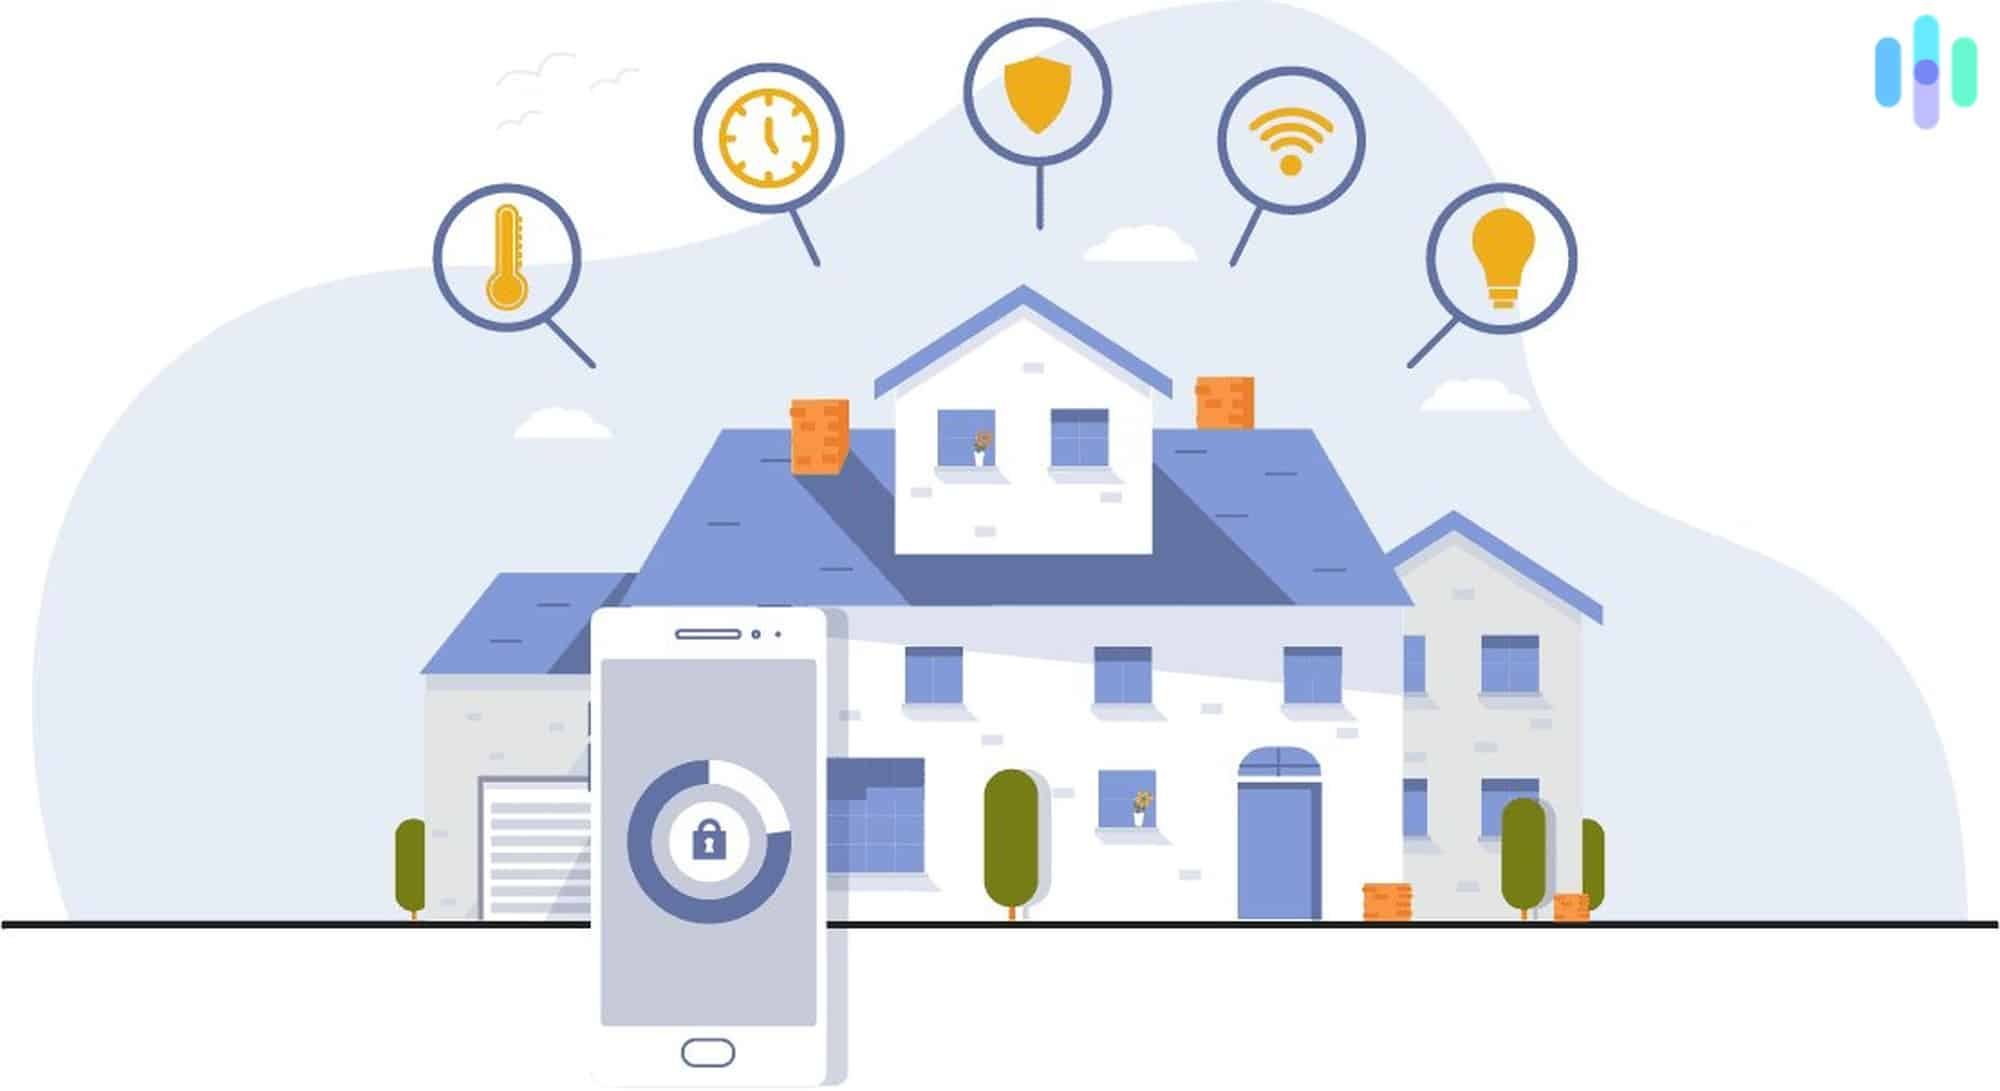
\includegraphics[width=70mm, keepaspectratio]{figures/What-is-a-Smart-Home.jpg}
    \caption{Smart home felépítése}
\end{figure}
\par Egy modern, intelligens, „okos” otthont különféle számítástechnikai és elektronikai eszközök, illetve vezeték nélküli érzékelők együttesen alkotják. Az automatizáció megjelenése során a felhasználók újabb és nagyobb elvárásokat követelnek, mely a felhasználókra szabott, fejlesztett automatizált rendszerek viselkedéséhez új utakat lehet törni. Az okosotthonok világa előtt, egy átlagos családnak közönséges betörőkkel, bűnözőkkel kellett szembe szállniuk, míg jelen pillanatban a fejlesztőknek és az okos otthonnal rendelkezőknek, számítástechnikában jártas, technikailag igencsak fejlett kiberbűnőzökkel kell felvenni a harcot, hogy megvédhessék otthonukat az esetleges külső támadásoktól. Ezek az emberek képesek megtalálni és kihasználni azokat a biztonsági réseket, amelyek alapján lehetőségük van manipulálni az adott hálózatot és az ahhoz csatlakoztatott eszközöket is, ezáltal könnyedén szabad utat nyerve a bejutáshoz. A lakatok és zárak fizikai feltörését felváltja például egy riasztórendszer tűzfalának kiiktatása vagy az automata kapunyitórendszer meg hackelése. Azonban az okosotthonok biztonsági kérdése kritikusan foglalkoztatott és fokozott figyelmet kap, viszont a technika mai állása szerint kijelenthetjük, hogy teljesen tökéletes és 100%-ig biztonságos rendszer nincsen. 
Számos kutatás és kísérletezés valósult meg az okosotthonok koncepciójával kapcsolatban az 1970-es évek vége óta. Fontos tényező, hogy mivel megfizethetőbbek és népszerűbbek lettek az elektronikus eszközök és az internethez való hozzáférés is. Hatalmas szerepet játszik az automatizálás és a kényelem, ezért egyre jobban érdeklődnek az emberek az okosotthonok iránt. 
\cite{smart-homes}